\documentclass[11pt]{report}

\usepackage{a4,fullpage}
\usepackage{enumitem}
\usepackage{setspace}
\usepackage{natbib}
\usepackage{array}
\usepackage{multirow}
\usepackage{pifont}
\usepackage{fancyhdr}
\usepackage[super]{nth}
\usepackage[letterspace=400]{microtype}
\usepackage{hhline}
\usepackage[table, dvipsnames]{xcolor}
\usepackage{listing}
\usepackage{listings, xcolor}
\usepackage{bold-extra}
\usepackage{float}
\usepackage{graphicx}
\graphicspath{{images/}}

% Allows for hyperlinking throughout document
\usepackage{hyperref}

% listing design
\newcommand\JSONnumbervaluestyle{\color{blue}}
\newcommand\JSONstringvaluestyle{\color{red}}

% switch used as state variable
\newif\ifcolonfoundonthisline

\makeatletter

\lstdefinelanguage{JavaScript}{
  keywords={typeof, new, true, false, catch, function, return, null, catch, switch, var, if, in, while, do, else, case, break},
  keywordstyle=\color{blue}\bfseries,
  ndkeywords={class, export, boolean, throw, implements, import, this},
  ndkeywordstyle=\color{darkgray}\bfseries,
  identifierstyle=\color{black},
  sensitive=false,
  comment=[l]{//},
  morecomment=[s]{/*}{*/},
  commentstyle=\color{purple}\ttfamily,
  stringstyle=\color{red}\ttfamily,
  morestring=[b]',
  morestring=[b]"
}

\lstdefinestyle{json}
{
  showstringspaces    = false,
  keywords            = {false,true},
  alsoletter          = 0123456789.,
  morestring          = [s]{"}{"},
  stringstyle         = \ifcolonfoundonthisline\JSONstringvaluestyle\fi,
  MoreSelectCharTable =%
    \lst@DefSaveDef{`:}\colon@json{\processColon@json},
  basicstyle          = \ttfamily,
  keywordstyle        = \ttfamily\bfseries,
}

% flip the switch if a colon is found in Pmode
\newcommand\processColon@json{%
  \colon@json%
  \ifnum\lst@mode=\lst@Pmode%
    \global\colonfoundonthislinetrue%
  \fi
}

\lst@AddToHook{Output}{%
  \ifcolonfoundonthisline%
    \ifnum\lst@mode=\lst@Pmode%
      \def\lst@thestyle{\JSONnumbervaluestyle}%
    \fi
  \fi
  %override by keyword style if a keyword is detected!
  \lsthk@DetectKeywords% 
}

% reset the switch at the end of line
\lst@AddToHook{EOL}%
  {\global\colonfoundonthislinefalse}

\makeatother

\lstset{
  escapeinside={<@}{@>},
  showstringspaces=false,
  showspaces=false,
  numbers=left,
  numberstyle=\footnotesize,
  frame=single
}



\begin{document}

% fancy header at top of each page 
\pagestyle{fancy}
\setlength{\headsep}{0.8cm} % changes space at top of page

% allows for normal citing with this bib style
\setcitestyle{square,numbers}

% Defines tick and cross
\newcommand{\cmark}{\ding{51}}%
\newcommand{\xmark}{\ding{55}}%

% Allows centred paragraph cells in tables
\newcolumntype{P}[1]{>{\centering\arraybackslash}p{#1}}
\newcolumntype{M}[1]{>{\centering\arraybackslash}m{#1}}

% Allows for horizontal lines with custom thickness on title page
\makeatletter
   \def\vhrulefill#1{\leavevmode\leaders\hrule\@height#1\hfill \kern\z@}
\makeatother

\begin{titlepage}
    \begin{center}
        \vspace*{2cm}
        
\includegraphics[width=0.5\textwidth]{imperial_logo}
        \vspace{2cm}
        
        \LARGE
        \textsc{Department of Computing}
        
        \textsc{Individual Project Final Report}
        
        \vspace{2cm}
        \vhrulefill{2pt}
        \vspace{0.2cm}
        
        \huge
        \textbf{\textsc{Amble}}
        
        \vspace{0.2cm}
        
        \LARGE
        \textbf{A Social Walking App}
        
        \vspace{0.2cm}
        \vhrulefill{2pt}
        \vspace{2cm}
        
        \begin{flushleft}
            \Large
            \textit{Author:}
            \hfill
            \textit{Supervisor:}\\
            Jonathan \textsc{Muller}
            \hfill
            Professor Michael \textsc{Huth}\\
        \end{flushleft}
        
        \vfill
        \Large
        \today
    \end{center}
\end{titlepage}

% set size between paragraphs
\setlength{\parskip}{0.3cm}

\begin{abstract}

%Fitness applications have become increasingly popular to record workouts, an indicator of how important it is to exercise and keep fit. Research was conducted to find out the ways in which these applications try to engage the user to encourage them to exercise more, such as adding an element of gamification in an attempt to motivate the user.

In today's society, it is extremely important to try to keep fit and exercise. This can be seen by the increasing popularity of fitness applications over the recent years. The problem that is posed by fitness apps is to try to engage with the user in an attempt to motivate them to exercise more. Various methods were researched to try and solve this problem, in particular exercising in groups and using gamification, both of which were employed in this project.

This project aims to provide a means to encourage people to exercise more and discover more about the world around them. We have created an iOS application that allows the user track the walks they go on and view points of interest around them. We have also created a back-end API that the mobile app can interact with to store and retrieve user data.

We then tested and evaluated the application with real users to assess whether it had an impact on how often they exercise and whether they were able to discover new places in their area. The results obtained suggest that the application produced did have a positive impact on the user in the areas described above, but with a few limitations that could be improved on in the future.

\end{abstract}

\begin{spacing}{1.3}
  \tableofcontents
\end{spacing}
\newpage

\begin{spacing}{1.1}

  
  \chapter{Introduction}

\section{Motivation}

% Background - what is the problem?
% Why is the problem difficult to solve
% The idea which this project is solving

In this day and age, it is extremely important to keep fit. With the rapid development in technology in the recent years, people are more inclined to stay inside looking at a screen rather than to go outside and exercise. The main demographic seeing an increase in the use of smartphones and computers are teenagers and young people. The increased day-to-day use of technology is shown to have an impact on the number of obese adolescents in the UK \cite{Kautiainen2005}, which can increase the chances of people developing serious illnesses including diabetes \cite{Lazar2005}. It is therefore of great significance to provide a means of exercising that helps people, especially adolescents, keep healthy.

The difficulty in trying to encourage people to exercise lies in the ability to engage the user and find something that they enjoy to do. If exercising is seen as something that you enjoy, it then becomes a pleasure to do rather than a burden. Gamification plays an important part in helping people exercise, and has been used in lots of fitness apps available on the iOS App Store already \cite{Lister2014}. The range in which companies have implemented gamification into their fitness applications ranges from a score-based system where users can compete against their friends to a complete game that allows the user to explore the world around them. An example of the latter is the popular mobile game Pok\'{e}mon Go, where you have to walk around and capture virtual `creatures' that are scattered around in the real world.

Another problem in trying to keep fit is the difficulty of motivating yourself to exercise regularly. A study conducted in 2001 found that exercising with another person helped to reduce stress and increase calmness compared with exercising alone, however it also resulted in people being more tired \cite{Plante2001a}. As well as this, exercising with another person also allows you to motivate and set goals for each other to achieve, which can be a challenge when exercising by yourself.

The idea behind this project is to encourage people to walk more often via helping them to find out more about the area around them. Exploring your surroundings can be very interesting and walking is one of the best ways to discover new areas. Let's say, for example, that there is a monument along your commuting route. When travelling via another means of transport, such as a car or train, you might not have the chance to notice this monument. When walking, along with a tool which displays points of interest as you were walking, you would be able to see something that you may never have noticed before.

The idea also extends to helping people walk together to promote regular exercise. A way to do this is to allow the user to schedule walks for a point in the future, and invite their friends along to join them. This means that users will have a fixed event in their calendar that will help keep a more structured fitness routine.


\section{Objectives} \label{section:objectives}

The aim of this project is to produce a working application that encourages people to walk more and helps discover new places in the world. The main objectives for the project to measure success on are as follows:

\begin{enumerate}[label=\textbf{Obj \arabic*}]
  \item \textbf{Encourage walking:} users should be encouraged to keep fit and exercise more.  One way to do this is to make it easy for users to exercise with another person as it has been shown to increase motivation and reduce stress. Gamification is another method that could be used to encourage walking more. Users should be able to compete with their friends as a means of motivating one another.
  \item \textbf{Help discover the world:} while walking users should be able to discover new places or points of interest in the area around them, which will hopefully motivate them to explore new areas of the world as well as increasing their fitness at the same time.
  \item \textbf{Test and evaluate with real users:} evaluation should be conducted with real users to see if the project has an impact on how often they exercise.
\end{enumerate}

% add evaluation of project as objective, refer to evaluation plan section







  \chapter{Background} \label{chapter:background}

\section{Health Benefits}

\section{Existing Applications}

% overview

There are a number of existing applications available that attempt to solve the problem posed by this project. These range from fitness applications to various navigation applications, which although may not be completely relevant to this project, do provide some similar features such as place recognition that will be useful to research.

Table \ref{table:existing-walking-apps} shows how well each of the existing applications related to this project have implemented certain features. The maximum score for the feature category is displayed in brackets. The full matrix detailing what aspects each feature category is split into and why the score was given to each app can be seen in Appendix \ref{appendix:existing-apps-matrices}.

\begin{table}[htb]
  \centering
  \begin{tabular}{|m{2cm}||c|c|M{1.5cm}|M{1.5cm}|c|c|}
    \hline
    \textbf{Features} & \textbf{MapMyWalk} & \textbf{Strava} & \textbf{Let's Walk} & \textbf{Google Maps} & \textbf{Citymapper} & \textbf{Pok\'{e}mon Go}\\
    \hline
    \hline
    Design (2) & 1 & 2 & 0 & 2 & 2 & 2\\
    \hline
    Ease of use (3) & 3 & 3 & 1 & 3 & 3 & 3\\
    \hline
    Tracking location (2) & 2 & 2 & 2 & 1 & 1 & 1\\
    \hline
    Navigation (4) & 3 & 1 & 1 & 3 & 1 & 2\\
    \hline
    Social interaction (5) & 2 & 2 & 2 & 0 & 0 & 0\\
    \hline
    \hline
    Total (16) & 11 & 10 & 6 & 8 & 7 & 9\\
    \hline
  \end{tabular}  
  \caption{Matrix showing how well existing walking apps perform at given features. Each app is given a score for a category, with the maximum score shown in brackets next to the feature category.}
  \label{table:existing-walking-apps}
\end{table}

The rest of this section discusses each application in detail, explaining their benefits and limitations. All of the applications researched are free to use unless stated otherwise.

% go through each existing app, discussing why they are good/bad with images

\subsection{MapMyWalk}

MapMyWalk \cite{Map} is a popular fitness application for iOS and Android that allows you to track your walks and complete challenges to help you keep fit. You are able to track a walk as you go on one, or log a previous workout that you have done without the app. The app also provides a premium subscription for \pounds4.49 per month, which gives you the ability to monitor your heart rate and set training goals designed to help you walk more.

The area in which MapMyWalk lacks is social interaction. A user can publish a walk that they have previously tracked to their profile, but there is no real aspect of communication with other users other than adding each other as friends. There is also a limited level of gamification in the app, with challenges being the only option available to encourage a higher rate of fitness. Challenges can either be added by the user or chosen from a precompiled list, with the latter being fairly limited in the range of options to choose from.

\subsection{Strava}

Strava \cite{StravaInc.} is another fitness application that primarily focuses on running and cycling. It features a sleek user interface with similar functionalities as MapMyWalk. The journey view within the application can switch between either showing the map of your workout or a statistics screen as shown in Figure \ref{fig:strava}, visibly showing the time elapsed in the workout, the distance travelled and your average pace per kilometre. Strava also provides a premium subscription for \pounds5.99 per month, which features personalised coaching and advanced analysis of your workouts.

The setback of Strava is that you cannot track walks in the app as you are constrained to either running or cycling. With regards to this project, it performs well in allowing the user to record and share their workouts but it does not provide any features for the user to explore areas around them. This is expected given that it is a fitness application and does not cater for walking whatsoever.

\begin{figure}[hbt]
  \centering
  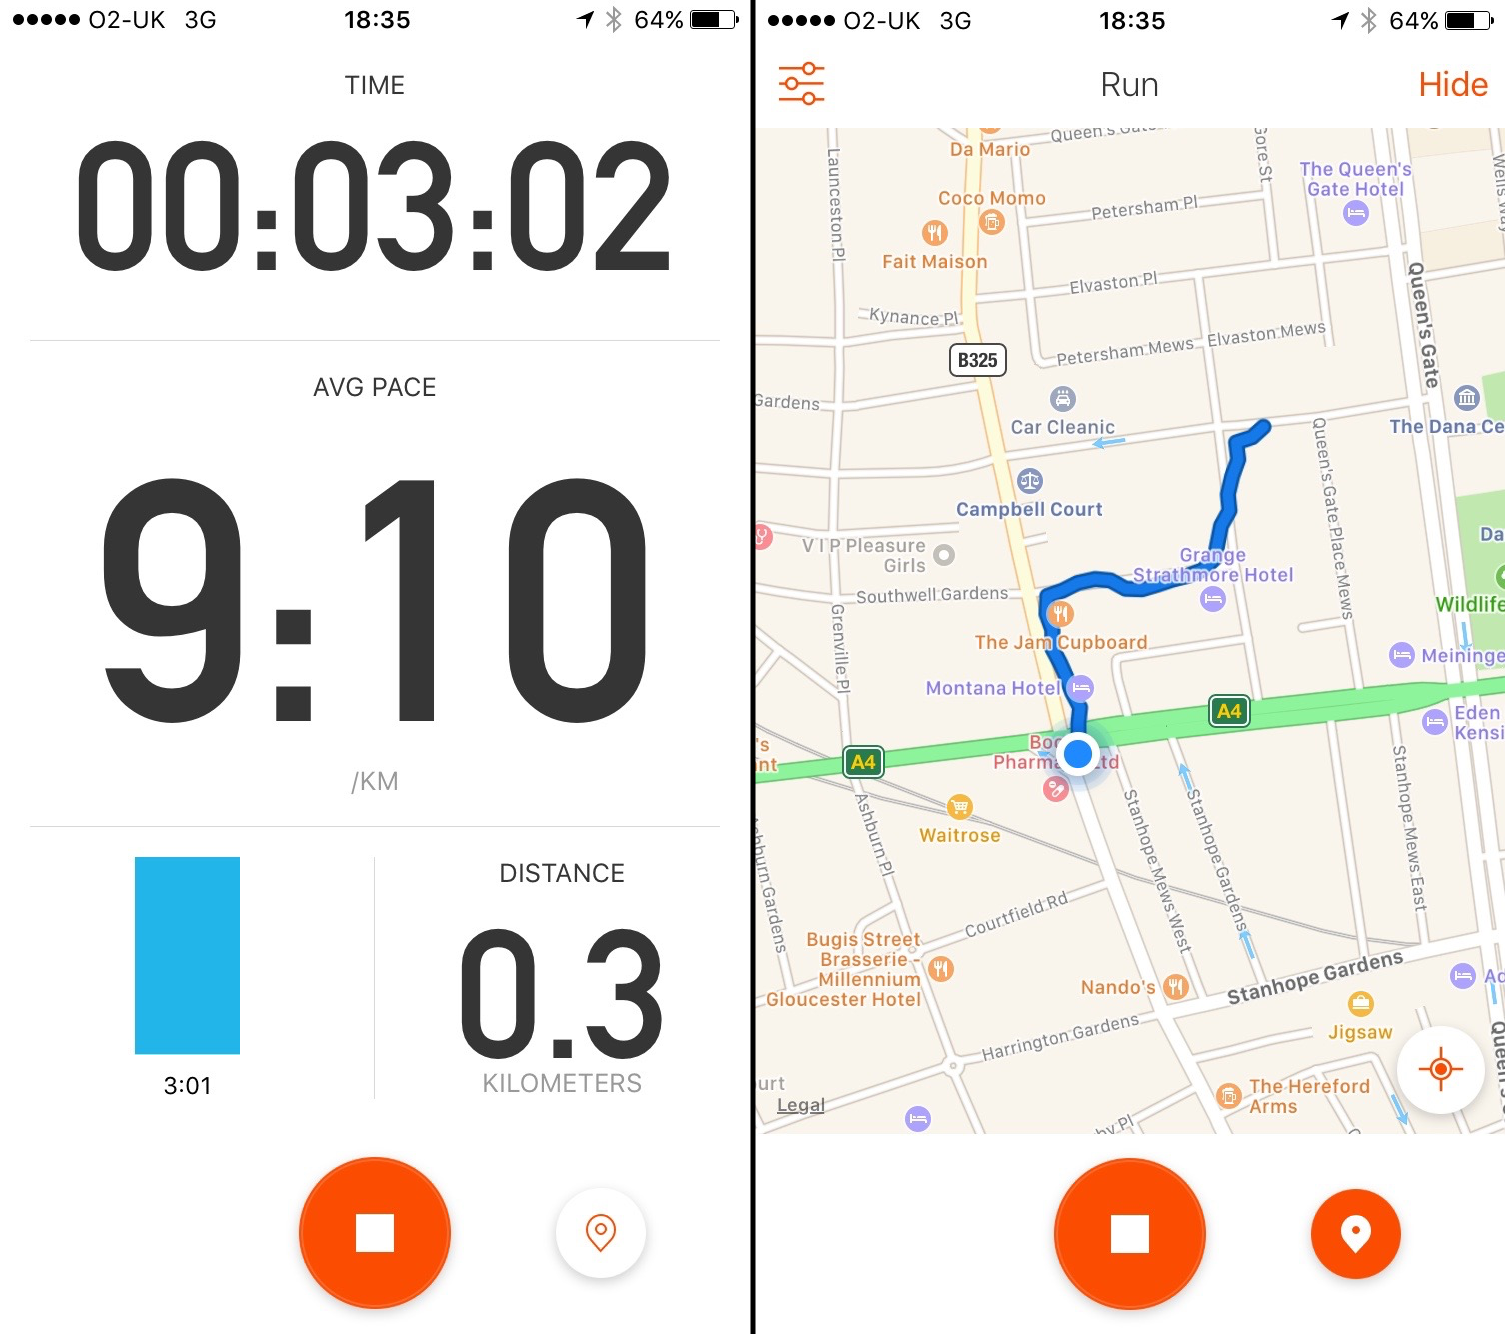
\includegraphics[width=0.7\textwidth]{strava}
  \caption{Journey view in Strava, allowing you to switch between statistics (left) or a map of your progress (right)}
  \label{fig:strava}
\end{figure}


\subsection{Let's Walk}

A lesser-known iOS fitness application is Let's Walk \cite{LetsWalkApp}. Users can record new walks and view a list of either their friends' walks or public walks nearby. The app is also focused on helping you maintain a balanced diet -- the amount of calories you consume can be added for particular meals during the day. A calorie goal per day can then be added, with the app recording how many calories were burned during a walk and updating the goal accordingly.

Let's Walk tries to emulate many of the features implemented by the more well-known apps as mentioned above, but a lot of these features seem unpolished. There is a global ranking section of the application showing which users have walked the most over the last week, month or year, however there seems to be little to do with this information other than view a leaderboard.



\subsection{Google Maps}

Although not a fitness application per say, Google Maps \cite{GoogleInc.} is one of the oldest services that provides route planning via different transport modes. The mobile app contains current information about public transport, traffic and displays well-known cycling routes on a map, however there is little in the way of customisation for walking. When entering a destination, the app generates a route but users can also choose from a few different routes on the map, with the app showing the difference in time each one would take. However, no information is given as to whether a certain route is quieter than another, for example.

\begin{figure}[hbt]
  \centering
  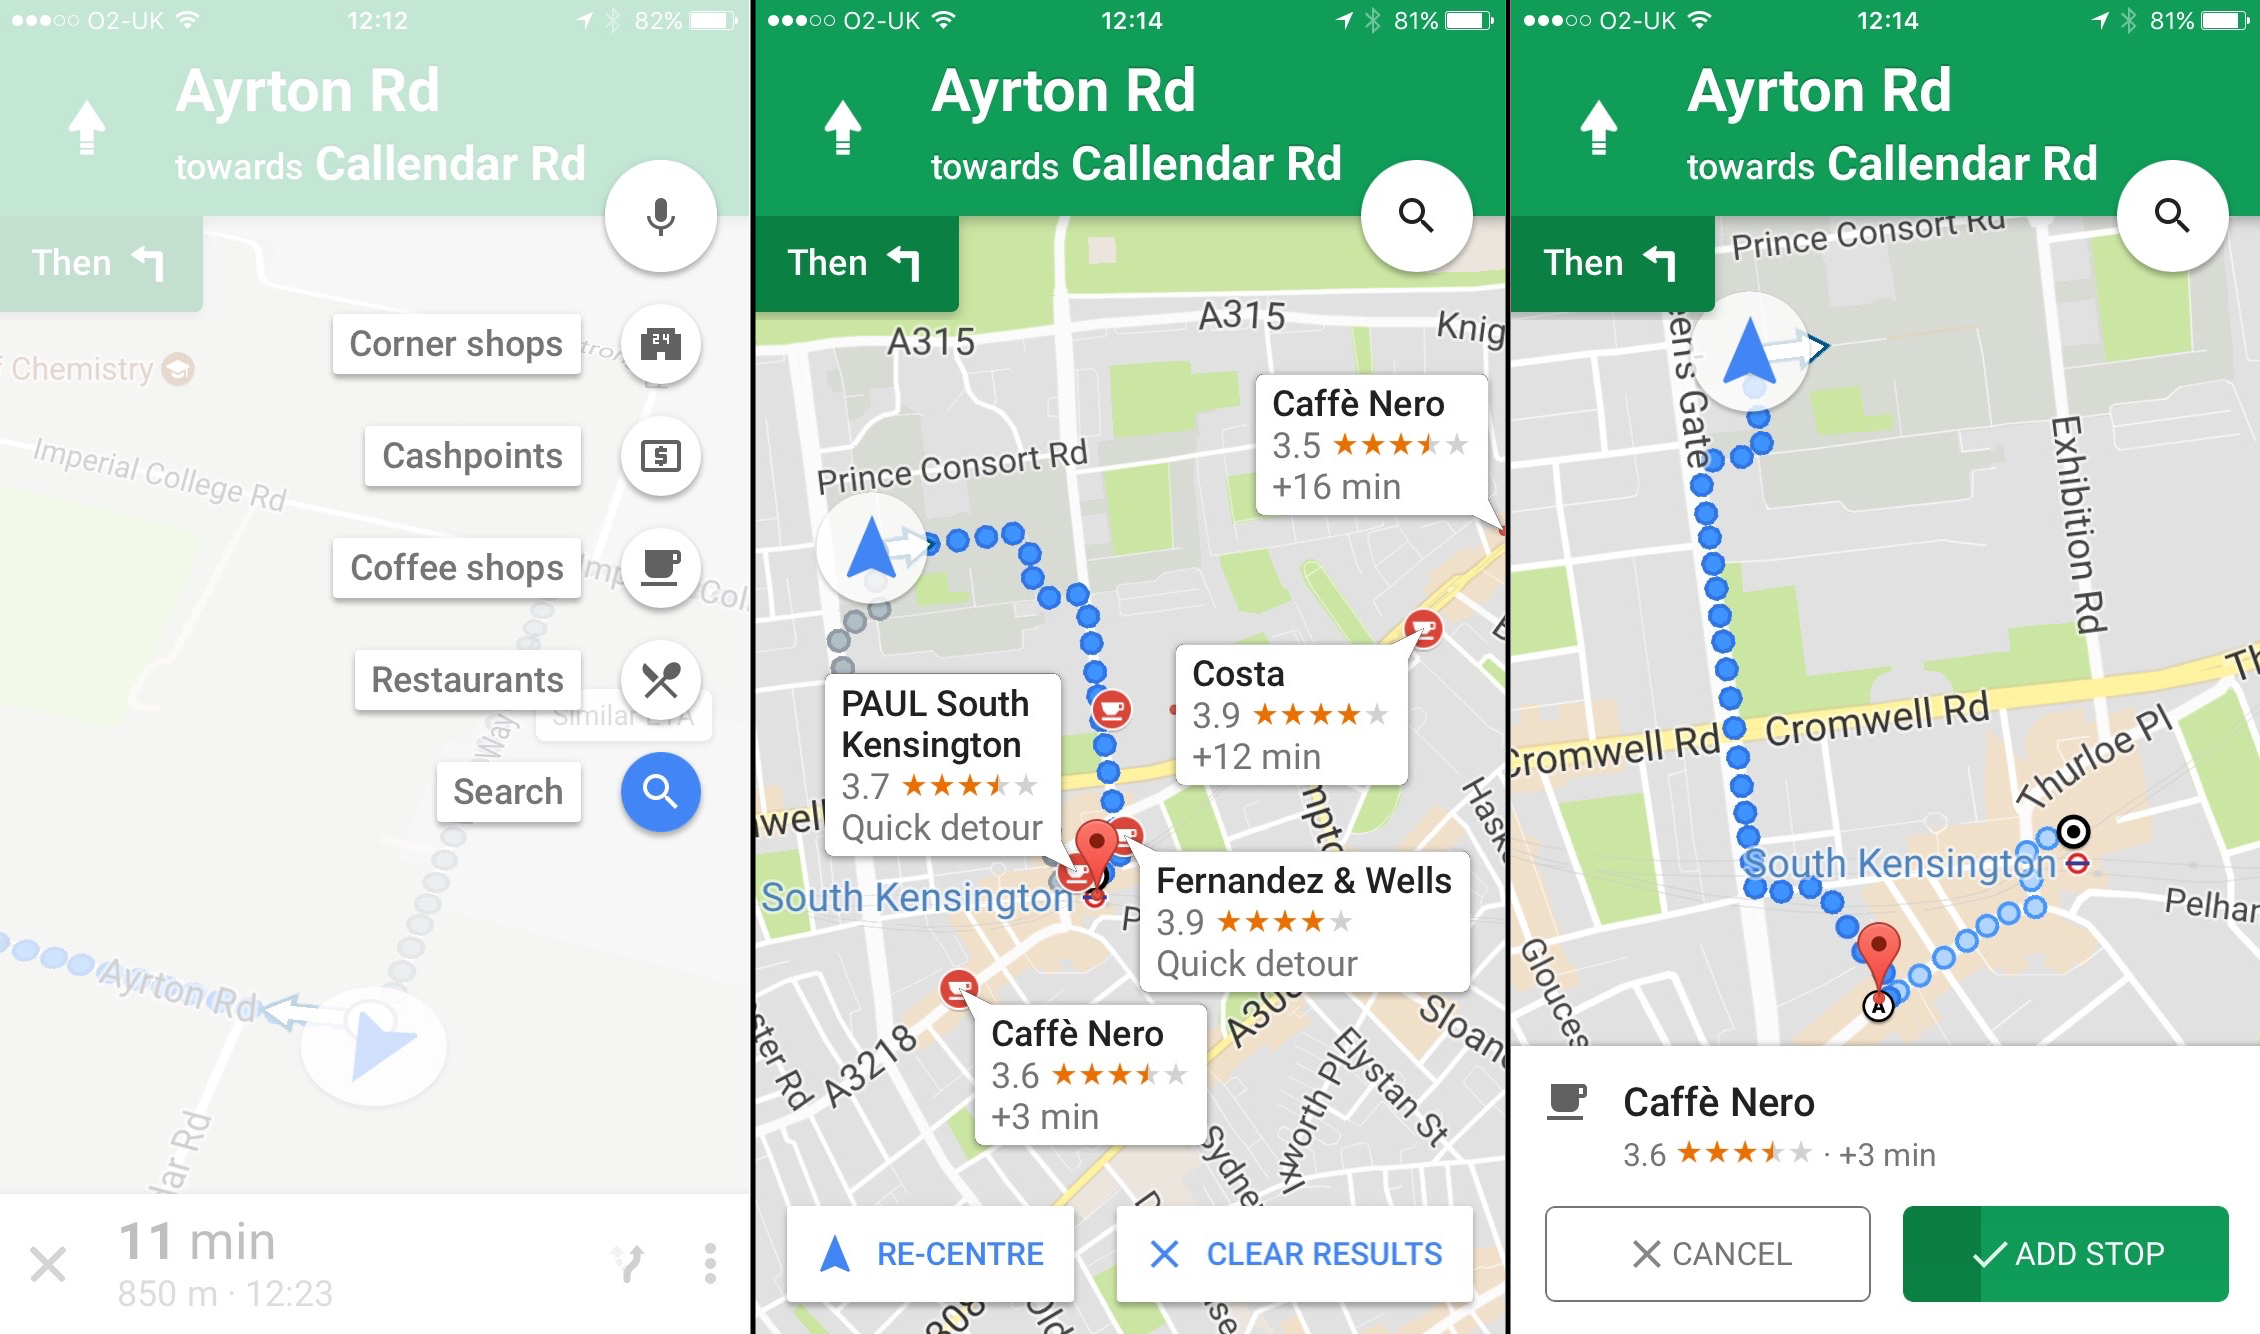
\includegraphics[width=\textwidth]{google_maps_place_search}
  \caption{Adding places along your walking route in Google Maps for iOS. A list of categories to choose from (left), then shows all the places from within a search on a map (middle). A stop can then be added and the journey will be updated (right).}
  \label{fig:google_maps_place_search}
\end{figure}


One feature of the Google Maps iOS application that is interesting to note is the ability to search for places along a route during a journey. Once a user has started a walking journey, they are able to search for places that are along the route. Google provides some categories of places to choose from, such as cashpoints and restaurants, but users can search for a specific place if they wish. The app will then display the results of the places search on the map, showing how much additional time would be added on to your journey if you were to stop at a place, if any. One or more places can then be added to your journey and the walking directions will subsequently update to include these new stops. Figure \ref{fig:google_maps_place_search} shows an example journey from Imperial College to South Kensington station. It details the full process of choosing \textit{coffee shops} as the place category, selecting a particular coffee shop on the map and the stop being added to the journey.

The places search feature is important as it is unique within any of the existing journey planner apps I have researched and it relates to one of my objectives regarding displaying points of interest when a user is on a walk (\textbf{Obj 2}). More research is conducted in Section \ref{subsection:background-apis} to discover what tools these applications use to implement this feature.

\subsection{Citymapper}

Originating in London, Citymapper \cite{Citymapper} has become one of the leading journey planners for major cities around the world including Paris, Barcelona, New York, Tokyo and Sydney. One of the key features of Citymapper is that different modes of transport can be combined to create a faster journey time. For example, a journey from Imperial College to Oxford Circus (as shown in Figure \ref{fig:citymapper}) could just use the Tube, but it could be faster to hire a bike and cycle to a different station and then take the Tube.

\begin{figure}[hbt]
  \centering
  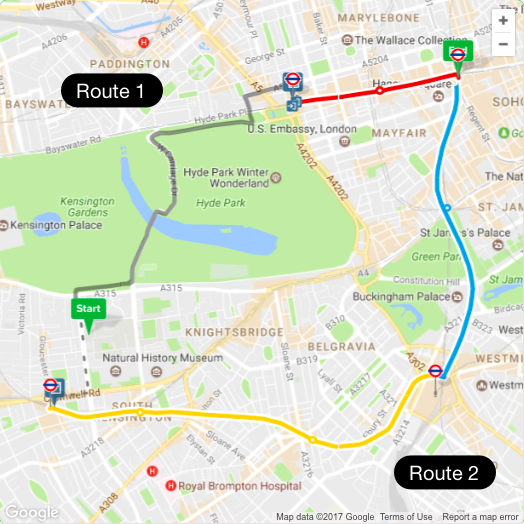
\includegraphics[width=0.7\textwidth]{citymapper}
  \caption{Two routes generated on the Citymapper website superimposed -- cycle and Tube route (Route 1) and Tube only route (Route 2)}
  \label{fig:citymapper}
\end{figure}

The walking directions in Citymapper are relatively limited. If you choose to walk on any route that you input, you are greeted with the screen shown in Figure \ref{fig:citymapper-walk}. Details such as estimated time of arrival, calorie burn and time of journey are displayed on this screen. Once you press \textit{Go}, you are transferred to the journey view, which simply tracks your location on a map and allows you to share your estimated time of arrival with others.

\begin{figure}[hbt]
  \centering
  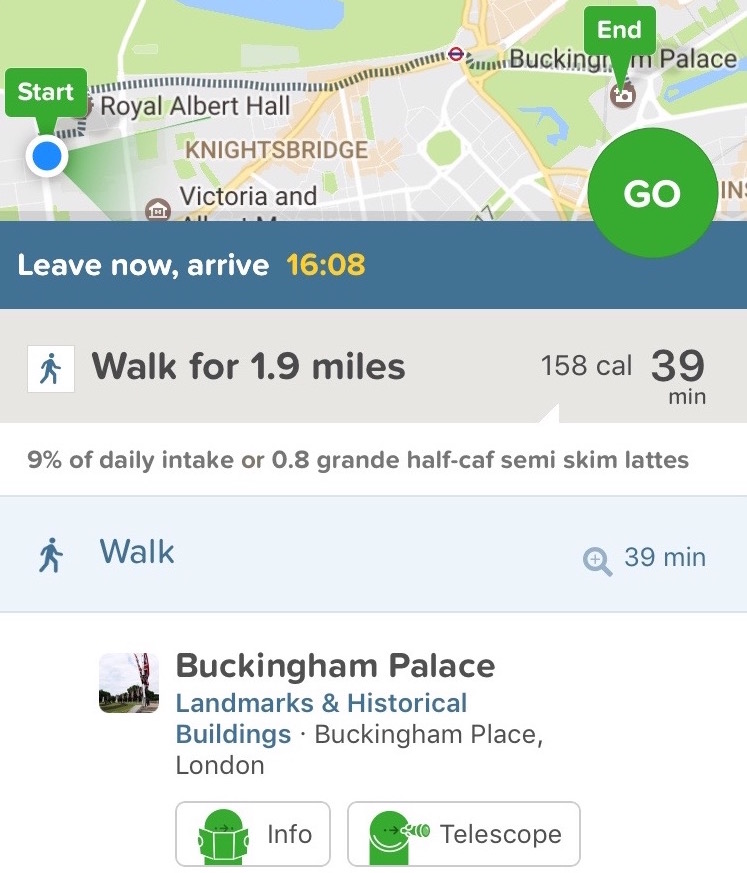
\includegraphics[width=0.55\textwidth]{citymapper_walk}
  \caption{Walking view in Citymapper}
  \label{fig:citymapper-walk}
\end{figure}

\subsection{Pok\'{e}mon Go} \label{subsection:pokemongo}

Pok\'{e}mon Go, released last July, quickly grew to become one of the most popular games of the year. Although not necessarily a walking application in the normal sense, the aim of the game is to capture virtual `creatures' called Pok\'{e}mon that appear in real world places. Thus, the game motivates you to walk more to collect more and more Pok\'{e}mon.

One of the more interesting parts of the application that is relevant to this project are the Pok\'{e}stops within the game. A Pok\'{e}stop is a location in the game where various in-game items can be collected. They are displayed on a map using blue beacons as shown in Figure \ref{fig:pokemongo}. These locations were crowdsourced by users of the game and are normally points of interest in the area such as a statue, a building or a famous plaque. Although not completely, this feature of the application does somewhat tie into my objective for helping people discover the world (\textbf{Obj 2}).

\begin{figure}[hbt]
  \centering
  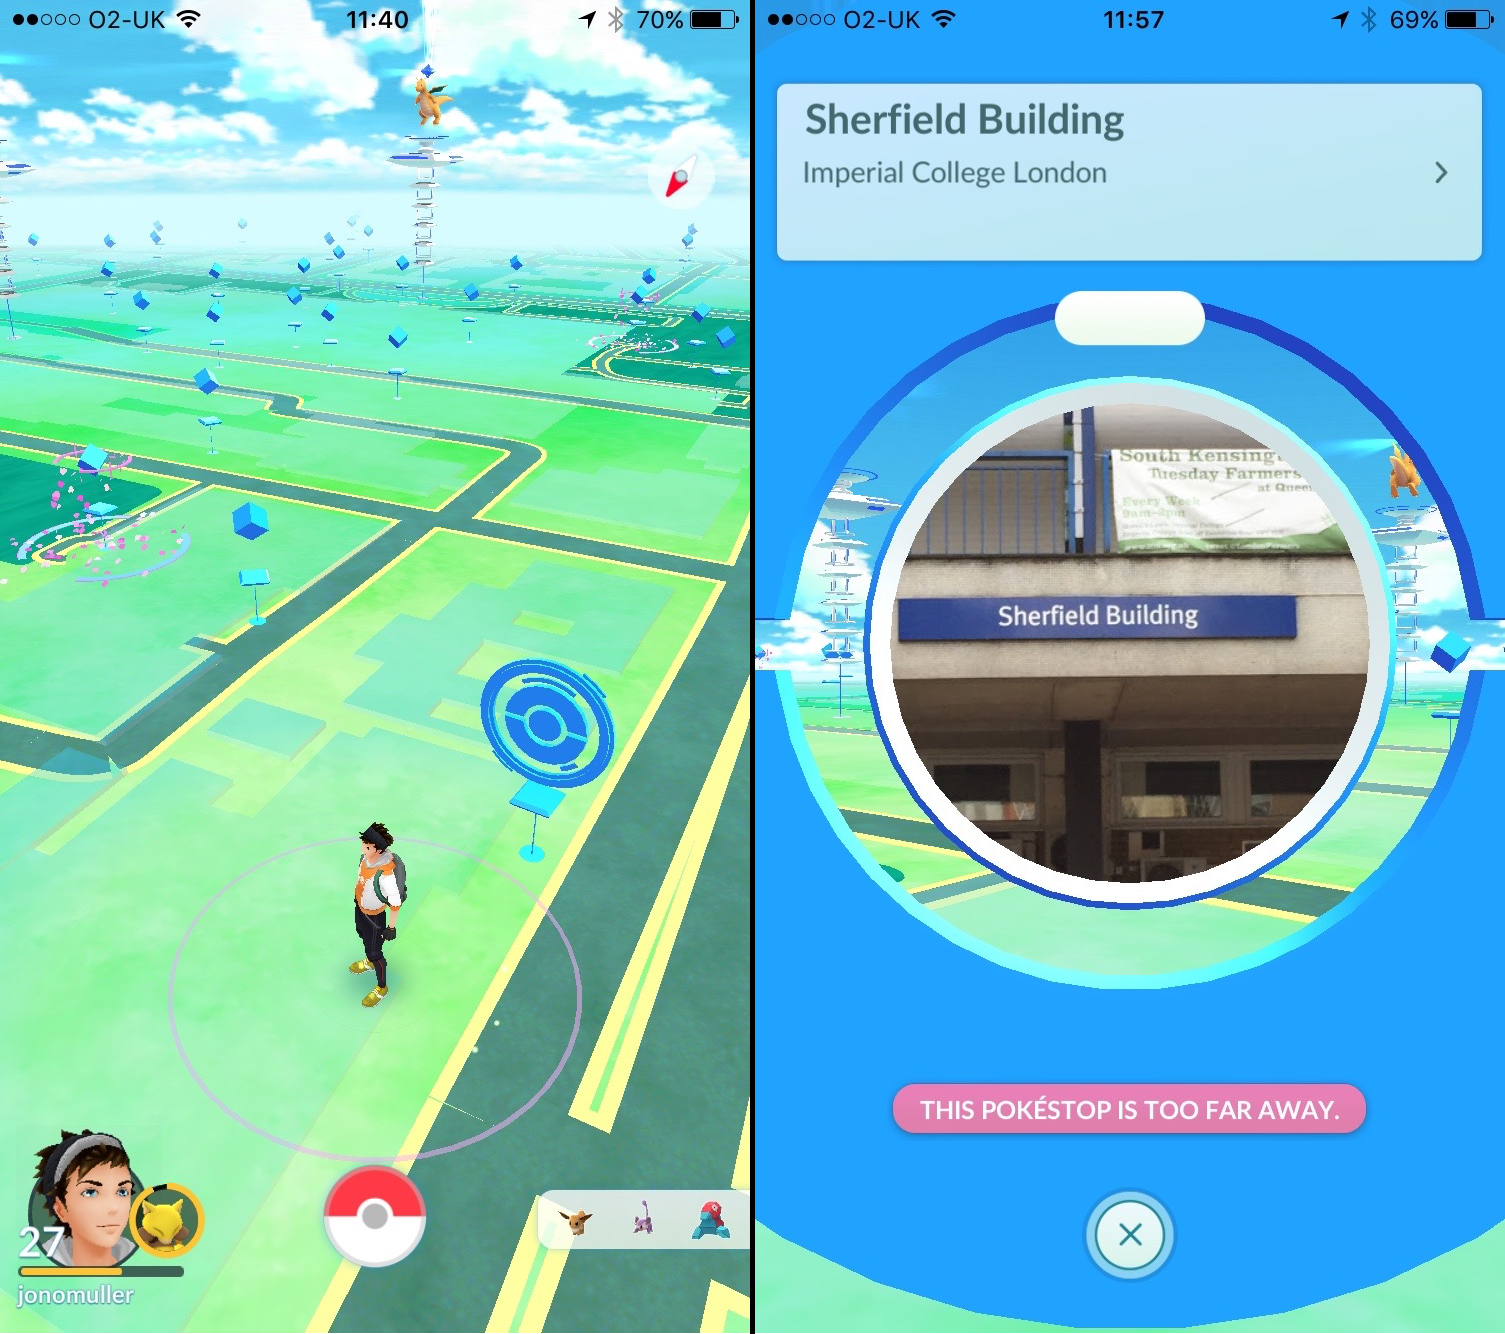
\includegraphics[width=0.7\textwidth]{pokemongo}
  \caption{Screenshots of Pok\'{e}mon Go showing Pok\'{e}stops in an area (left) and a detailed view of a Pok\'{e}stop (right)}
  \label{fig:pokemongo}
\end{figure}

\subsection{Summary}

From the subset of fitness applications that I researched in this section, it can be seen that some of the objectives I proposed in Section \ref{section:objectives} have been achieved but no single application encompasses all of my proposed objectives. I have found that it is important for this project to have a sleek design and easy-to-use interface as this is something that stood out straight away when looking at existing applications.

%\pagebreak

\section{Gamification}

% research how gamification has been used in applications, not just walking apps
% discuss how well each implementation has worked

Gamification is used in mobile applications not only for fitness but also in a wide range of areas including productivity, finance and mental health. We have seen how gamification can be used in existing fitness applications, with some apps setting challenges for users to complete within a given timeframe -- such as running a half marathon in February.

An application and website called Habitica \cite{Habitica}, labelled as a ``gamified task manager", helps motivate you to complete household tasks by unlocking features and levelling up an in-game avatar. Completing real-life tasks earns you gold for your character, which can then be redeemed for either virtual rewards such as equipment or real-life treats like watching an episode of a TV show, for example. The home page of Habitica, shown in Figure \ref{fig:habitica}, is split into columns containing your bad habits, daily tasks, to-do list and rewards. It also shows the progress of your avatar, along with what is needed to progress to the next level. This type of app helps you become more productive at home in a fun and creative way that users enjoy.

\begin{figure}[hbt]
  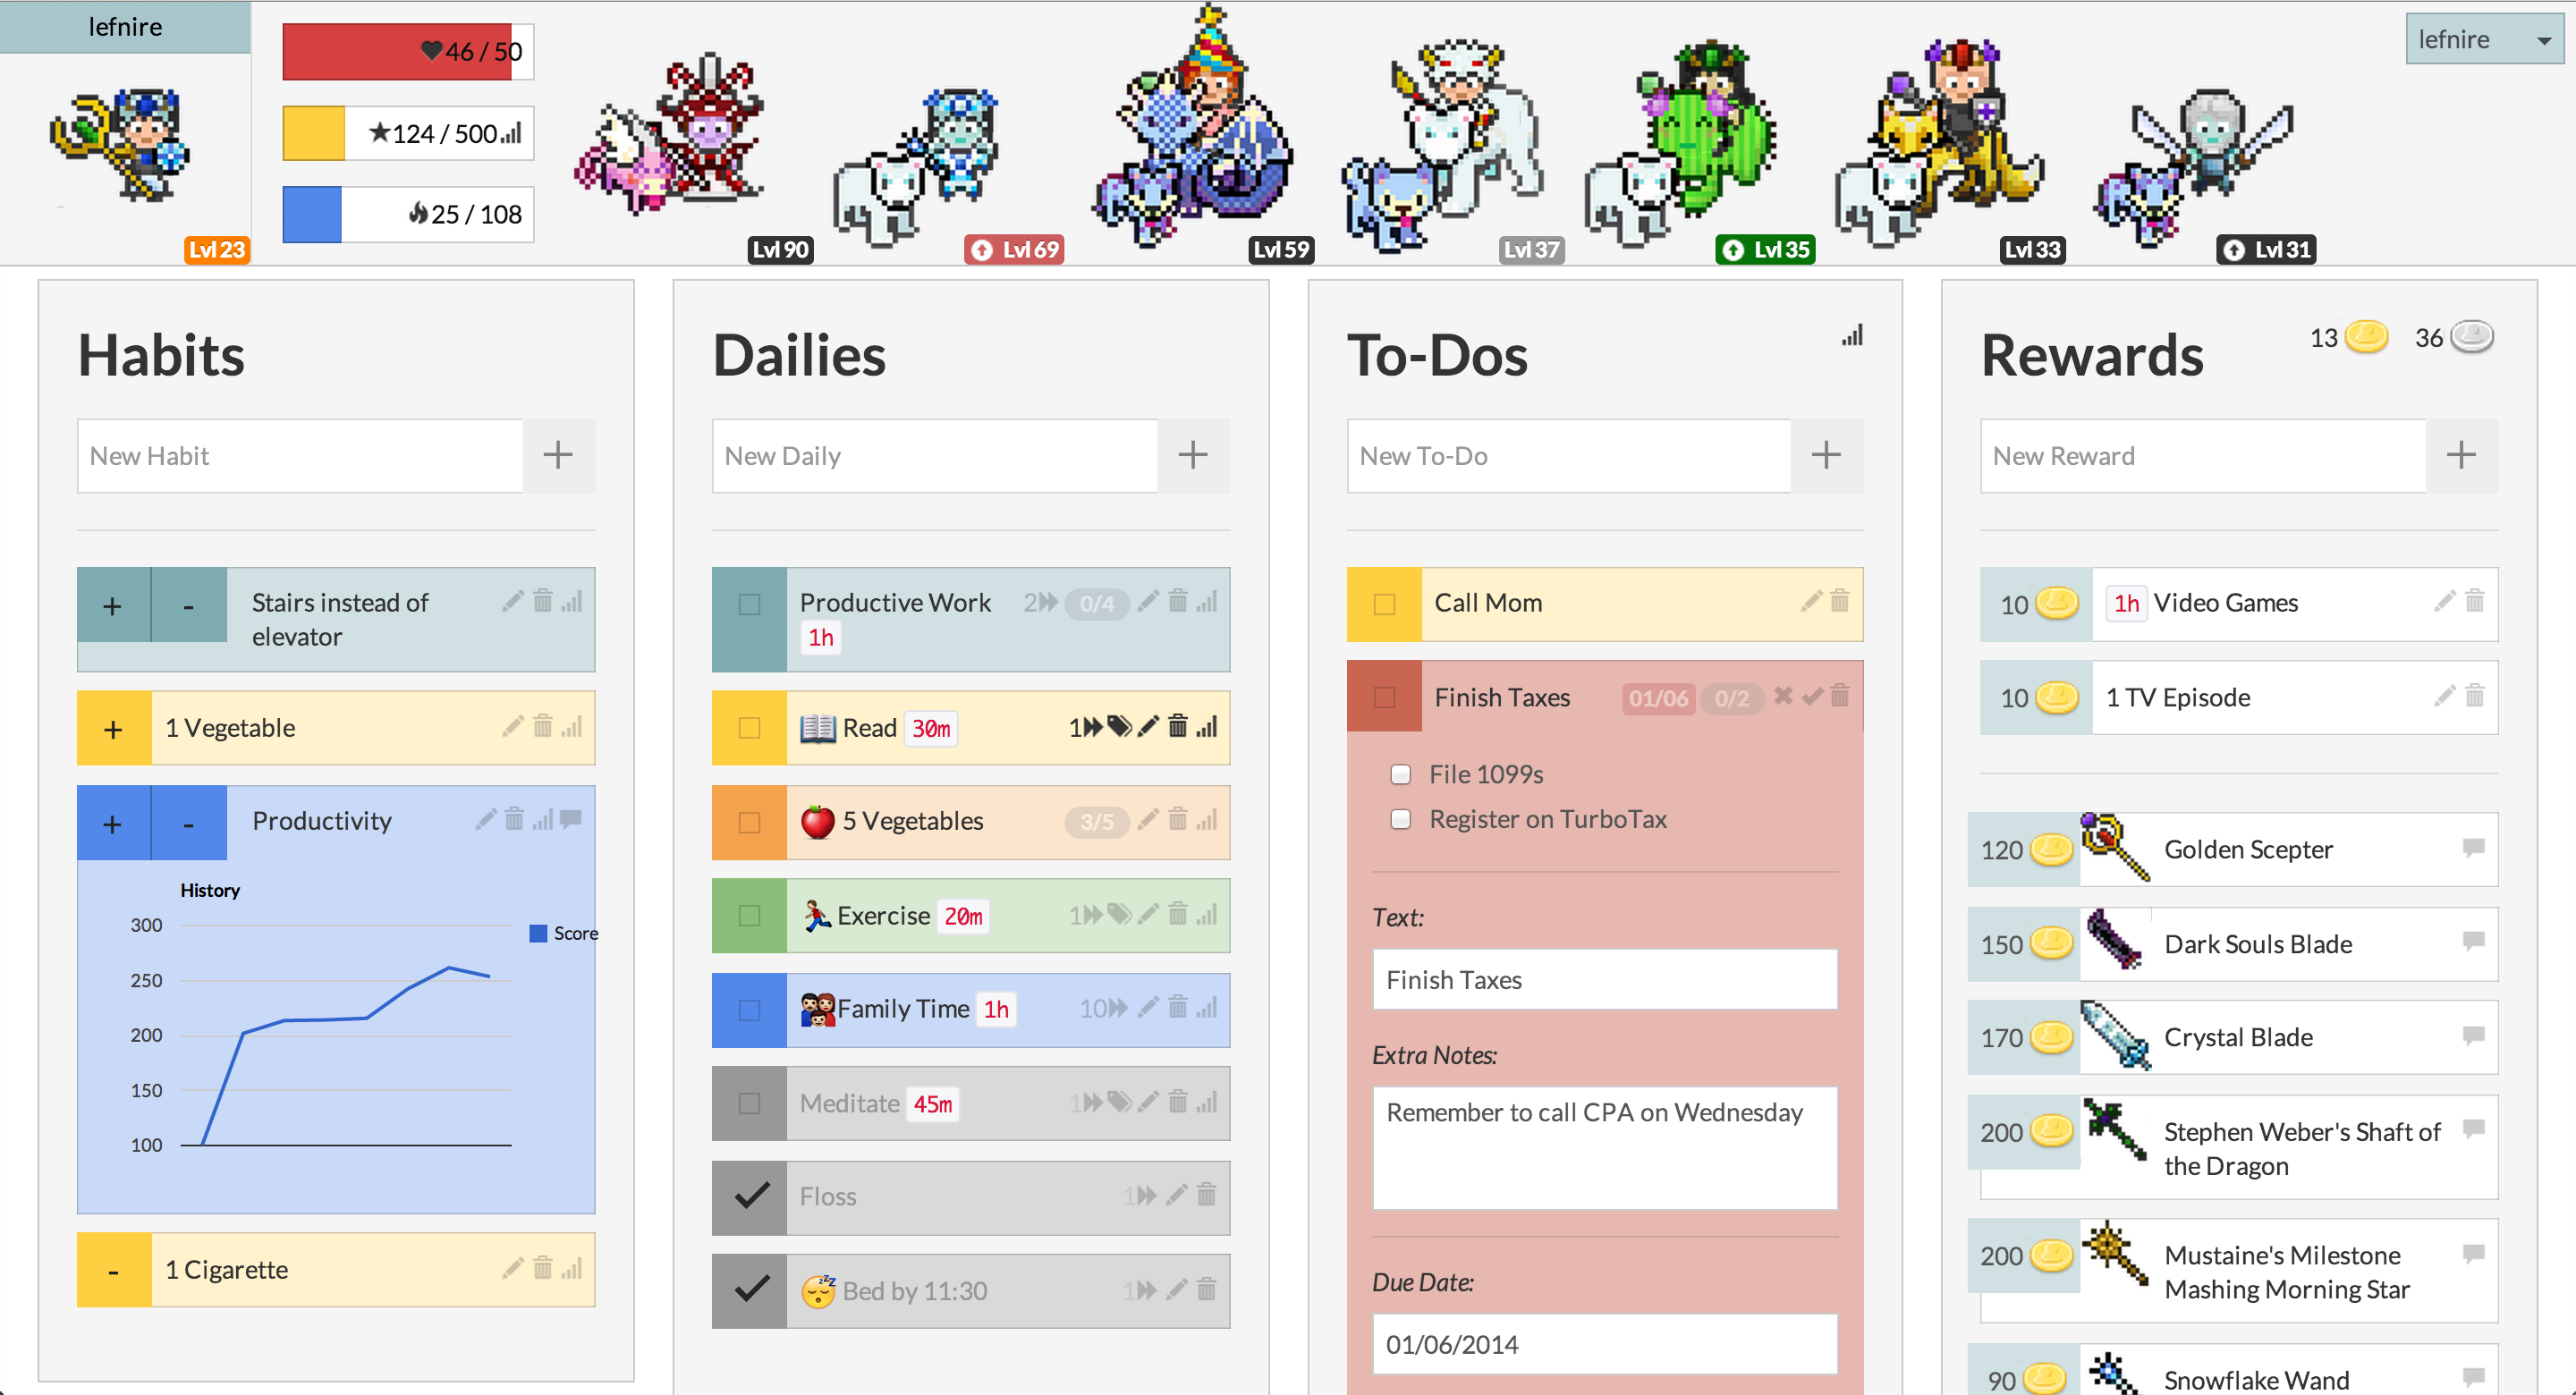
\includegraphics[width=\textwidth]{habitica}
  \caption{Home page of Habitica showing your habits, tasks and rewards as well as your avatar at the top \cite{Habiticaa}}
  \label{fig:habitica}
\end{figure}


Gamification is also used in some finance applications. Mint \cite{IntuitInc.} is an application available in America that links to your bank accounts to help you manage your bills and track how much money you spend. It shows a breakdown of what you are spending your money on and creates a budget with the option of using any left over money on goals designed to help you save money, as shown in Figure \ref{fig:mint}. You can create goals to be either a long-term one-off payment -- buying a house, for example -- or a short-term monthly payment such as a subscription service. This game mechanic of working towards a goal to help you buy something you want is extremely effective and is why gamification is so widespread.

\begin{figure}[hbt]
  \centering
  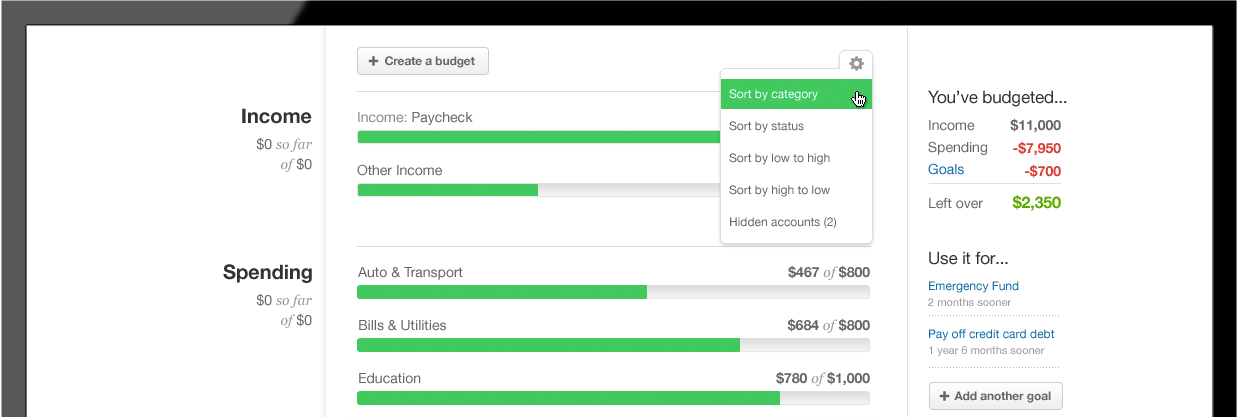
\includegraphics[width=\textwidth]{mint}
  \caption{The breakdown of spending in Mint, giving you the option to use any left over money from your budget for one or more goals \cite{IntuitInc.a}}
  \label{fig:mint}
\end{figure}

The idea of using gamification in applications is to motivate you to complete some form of task that you otherwise might not have attempted. It can make an app seem more engaging to the user, providing them with something to achieve every time they use the app. It is especially useful in fitness applications as keeping fit and staying healthy is very important, and should therefore be carefully considered for this project.

%\pagebreak

% not sure whether to include this in background or design?
% think I will include general background on technologies here, and then which ones I chose in design
\section{Technologies}

The features of existing applications are not the only important part to research -- the technologies that they use to implement these features are just as useful. This section discusses how existing applications implement certain features and which technologies integrate well with each other.

\subsection{Mobile Operating System}

Many of the applications that I have researched have been developed for iOS, the operating system running on iPhones and iPads. I have chosen to develop my application on iOS due to my previous experience with iOS app development. Another factor in this choice is that I have gained a lot of experience programming in Swift, one of the programming languages used to develop iOS apps, over the last few years. Swift is extremely readable and easy to use, which is the reason why I am choosing to use it over the other programming language available, Objective-C.

\subsection{Version Control} \label{subsection:version-control}

Version control is a crucial part of the development process with any project, especially this implementation-heavy project. It provides a full history of changes made to a codebase along with the ability to revert back to previous versions of code and work simultaneously on different features by creating branches. Git and GitHub are my chosen version control system and platform respectively due to past experience and familiarity.

Along with version control, errors or bugs in code must be detected quickly in order to not hinder the development process. To do this, the practice of continuous integration (CI) was used to integrate and test code frequently, making it easier to locate the origin of an error. There are many CI tools that can be used to automate code testing including Jenkins, Travis CI and BuddyBuild. I had no prior knowledge with any of these tools and so I researched the benefits and drawbacks of each service, which can be seen in Table \ref{table:ci-tools-options}.

\begin{table}[hbt]
  \centering
  \begin{tabular}{|m{1.5cm}||M{3cm}|M{3cm}|M{3cm}|M{3cm}|}
    \hline
     & \textbf{Jenkins} & \textbf{Travis CI} & \textbf{BuddyBuild} & \textbf{GitLab CI} \\
    \hline
    \hline
    Platform & Windows, macOS, Linux & Hosted & Hosted & Hosted on GitLab\\
    \hline
    Cost & Free & Free for students & \~\pounds55/month or free trial & Free for small individual projects\\
    \hline
    Main Feature & Plugins available for variety of languages & Linked well with GitHub & Designed solely for mobile development & Integrated with GitLab\\
    \hline
    Platform Specific & No & No & Yes & No\\
    \hline
  \end{tabular}
  \caption{Comparison of continuous integration tools}
  \label{table:ci-tools-options}
\end{table}

I concluded that Travis CI was most suitable option for me since it was hosted on GitHub and is not platform specific, meaning that I could use it to test both the mobile app and API even though they were written in different languages. Using an option like BuddyBuild could only be used for the mobile app, with another tool needed for the API.

\subsection{Location Tracking}

To track the user's location within iOS, an application can use the classes from the Core Location framework \cite{AppleInc.} inbuilt into the iOS SDK (software development kit). This framework allows a developer to obtain the user's current location in the form of latitude and longitude. To keep a history of where the user has been, these coordinates could be stored in an array and updated every few seconds. This will be useful for my application to show on a map where a user has previously walked.

% section on how to track calories burned?

\subsection{Map APIs} \label{subsection:background-apis}

One of the most important application programming interfaces (APIs) to consider is which source of map to use. The majority of existing applications use Apple's maps apart from, of course, Google Maps. This is because Apple's MapKit framework \cite{AppleInc.a} is much better integrated with the Core Location framework mentioned above, making it much easier to display the user's location on MapKit than on the Google Maps SDK. It also provides convenient functions for coordinate conversions and calculating distances between two coordinates, which is useful for this project when trying to calculate the distance of a tracked walk.

% maybe don't include
However, there are some advantages of Google Maps over Apple Maps -- one being that Google Maps tends to be more detailed than Apple Maps. An example of this is shown in Figure \ref{fig:google-apple}, where in my opinion roads are easier to see and buildings are clearly visible on Google Maps than on Apple Maps.

\begin{figure}[hbt]
  \centering
  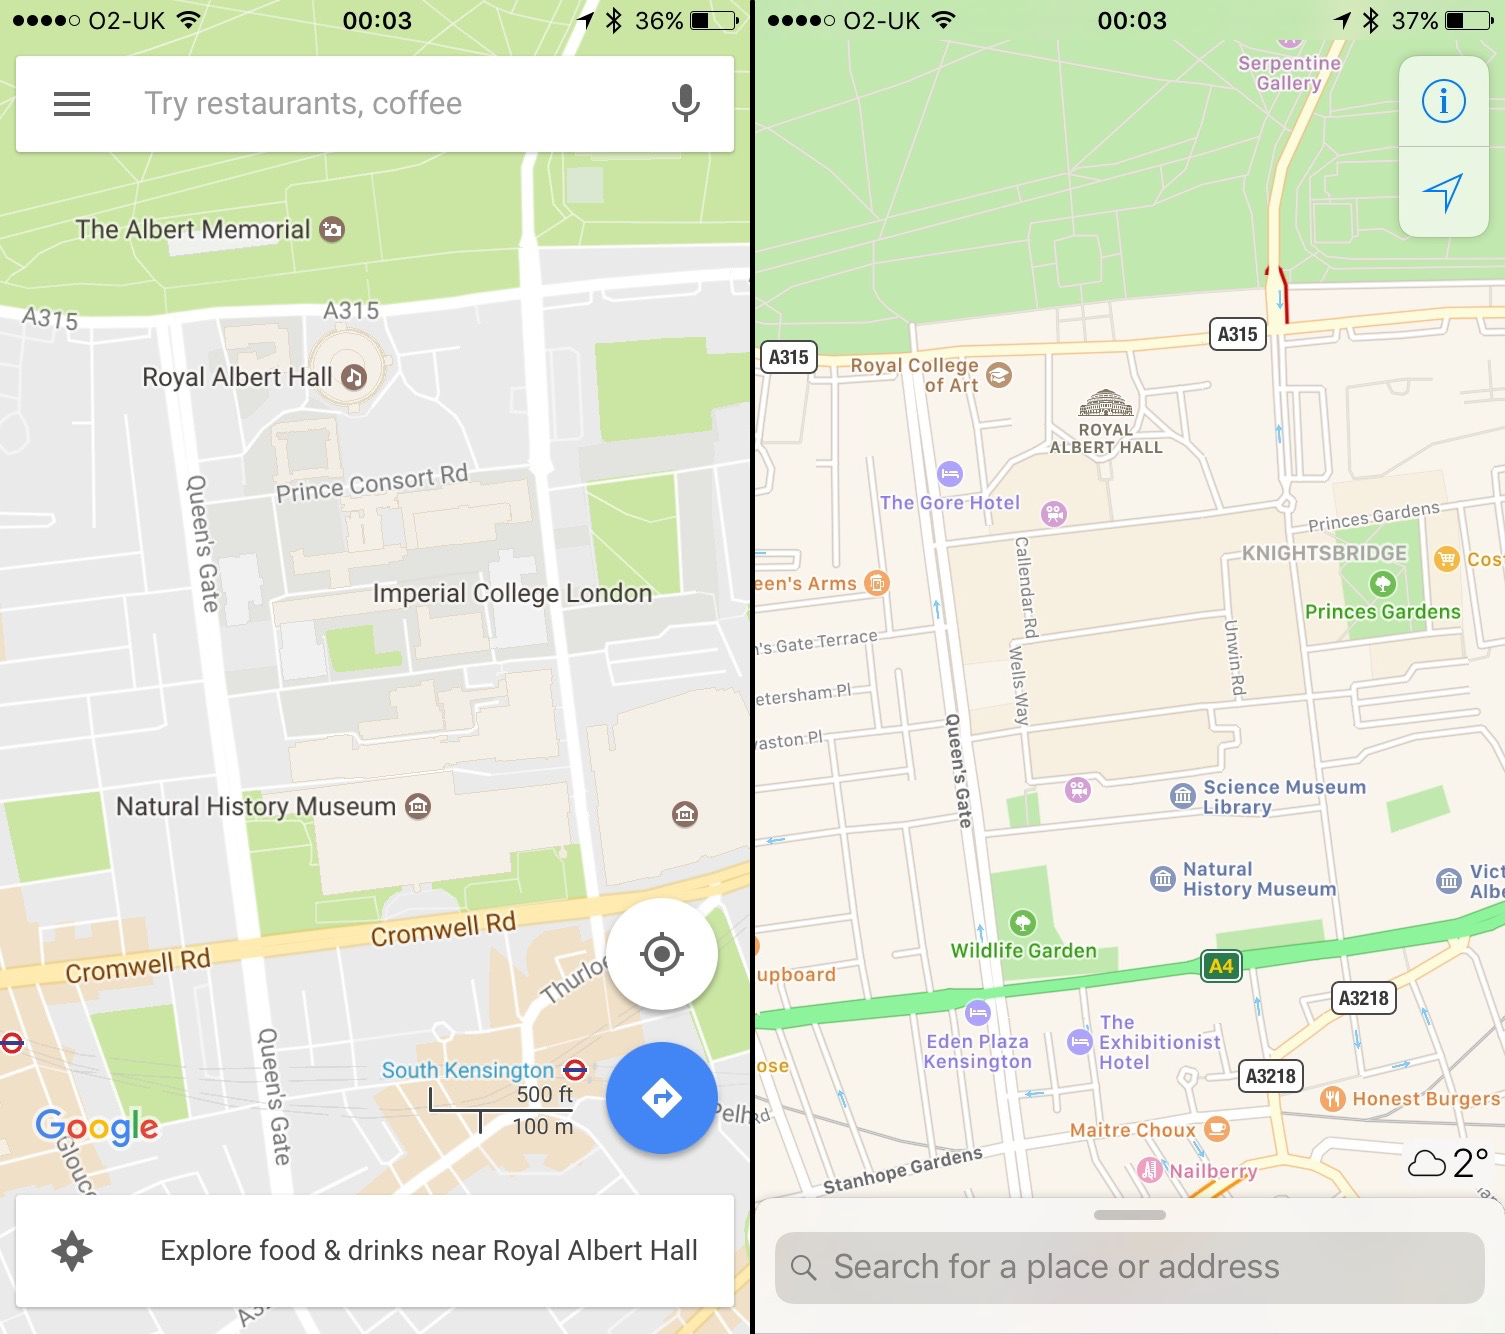
\includegraphics[width=0.7\textwidth]{google-apple}
  \caption{An example of the difference between Google Maps (left) and Apple Maps (right), showing Imperial College London}
  \label{fig:google-apple}
\end{figure}

%As discussed in Section \ref{subsection:background-apis}, Apple Maps very well integrated with the Core Location framework in iOS, which makes it easier to deal with displaying the user's location on a map. 

For the reasons listed above, I chose to use Apple Maps and their MapKit framework as the source of maps within the application. The one issue that I previously discussed with using this framework over Google Maps was the lack of detail in some areas of the maps. This factor was not deemed important enough to impact my decision and did not outweigh the benefits of the MapKit framework that are listed above.

\subsection{Place APIs}

The other API that I need to consider is one that gathers points of interest near a user's location. Google's Places API \cite{GoogleInc.b} would be a very good resource to use, allowing you to search for places by over a hundred types including \textit{point of interest}, \textit{place of worship} and \textit{museum}. The only issue with using Google Places is that you must use Google Maps to display the places on. From the Google Places Policies, \textit{``If your application displays data from the Google Places API for iOS on a map, that map must be a Google map"} \cite{GoogleInc.c}. This would mean that if I were to choose Apple Maps for the maps within the app, I would be unable to use Google Places as well.

Apple also provides an API for obtaining places called \texttt{MKLocalSearch} \cite{AppleInc.b}. To generate a list of places, you pass the \texttt{init()} method a \texttt{MKLocalSearchRequest}, which contains a string describing what type of place you would like to search for on a map. There seems to be little documentation online explaining what range of places that this API returns, which is something to consider when comparing it to other similar services.

A different option that could be used to generate points of interest around a geographical location originates from Pok\'{e}mon Go. As mentioned in Section \ref{subsection:pokemongo}, Pok\'{e}mon Go contains thousands of Pok\'{e}stops -- crowdsourced points of interest from all over the world. There exists an API \cite{Selwyn} that returns a list of Pok\'{e}stops in JSON format given a location. Each item that the API returns contains the name and location of a point of interest as shown in Listing \ref{listing:pokestop}, and so could therefore be used in this project.

\medskip

\begin{listing}
  \centering
  \begin{lstlisting}[style=json]
  {
      "distance": 44, 
      "name": "Sherfield Building", 
      "bearing": 200, 
      "latitude": 51.498359, 
      "image": "http://lh3.googleusercontent.com/07q4ms3tgDKsQMy04xye
            <@\textcolor{red}{\hspace*{20pt}\_i-UiraPO3jOS18TXwKpTMecgIXm2jXByO1CAUWVW9vNgqfx12ZtjqLdZrOlfsPu}@>", 
      "guid": "2cc0f9d9c7ba49348299c15749c49ea1.16", 
      "compass": "S", 
      "longitude": -0.178544
  }, 
  \end{lstlisting}
  \caption{Example of one item returned from the Pok\'{e}stop API, with attributes including its name, latitude, longitude and distance from your location}
  \label{listing:pokestop}
\end{listing}

% add section on blue plaque API
% used based on data from research survey


%\section{Technology Choices}

%The first part of the design of the project is to consider which technologies to use. The technologies that I chose stemmed either from the background research I conducted in the previous section or previous personal knowledge.

%\subsection{Mobile Operating System}

% move section in background to here?


% *** points of interest APIs ***

\subsection{Server Architecture} \label{subsection:server-architecture}

Before deciding what technologies to use for the server, such as which programming language to use, we must consider the type of architectural style to use. The aim of the API exposed by the server is to provide an abstraction between complex database queries and provide functionality that a client can use to query and update details. The Representational state transfer (REST) architectural principle fit the needs for this aim very well. Every component in a RESTful web service is a resource that can be accessed via the standard HTTP methods such as \textit{GET}, \textit{POST} and \textit{DELETE}. In comparison with other web services, such as the Simple Object Access Protocol (SOAP), RESTful services have much less overhead when sending data due to the extra XML header information sent when using SOAP.

With the architecture chosen, I assessed the options for the language to write the API in. There are a wide range of programming languages that could be used, and it came down to personal preference and how well it would suit the needs for this project. The popular options include PHP, Ruby, Python and Node.js ***ref*** -- the server-side environment run in Javascript. The only language in this list that I have experience in is Python, which would mean I would have to spend less time learning the language if I were to choose it. However, the advantage of Node.js for the purpose of this project is that objects in Javascript are built using Javascript Object Notation (JSON).

 RESTful web services support the use of multiple different data formats to serialise responses from the server, including HTML, XML and JSON. By choosing Node.js as the server language and JSON as the data type, I was able to easily parse data from HTTP requests and send responses in JSON despite not having any previous experience with Javascript.

\subsection{Database}

There are two types of database that could be used -- relational or non-relational. Relational databases are based upon relational algebra where data is stored in tables with queries to this data in the form of Structured Query Language (SQL). Each table in a relational database normally identifies a type of entity, and each instance of that entity is uniquely identifiable so that it can be referenced in other tables. SQL therefore supports the querying of this data across multiple tables using relational operators such as joining two tables. The most used services to model data in a relational database are MySQL and PostgreSQL, with the latter providing support for storing arrays -- a useful feature for this project as the coordinates of a walk need to be stored.

The opposite of this data model is a non-relational, or NoSQL, database in which each data entry is stored as a JSON-like document. This approach has many advantages for this project, primarily the similar use of JSON to both store data and build objects from in Node.js. As a result, data can be queried or inserted directly from a network request without any type conversions. NoSQL databases also have the benefit of faster query speeds and the ability to scale data horizontally -- an important factor to consider when designing a database.

The leading service to use for managing document-based NoSQL databases is MongoDB. It was used in this project especially due to its similar use of Javascript and JSON, both of which are already employed in the Node.js API. I also used a popular object data modelling library, Mongoose ***ref***, which helped with validation and allowed me to define schemas for each of the type entities.

\subsection{API Deployment}

I opted to host my API on the platform as a service Heroku ***ref***, with the alternative being Imperial's Cloudstack service run by the Department of Computing. Having had little experience with either of these services, I learned that Heroku had certain features that gained itself an advantage over Cloudstack.

Heroku is integrated with GitHub very well, my chosen version control platform, supporting automatic deployment when commits are made that can also be dependent on the results of continuous integration tests. Heroku also has a number of add-ons that can be used on web applications, including mLab -- a cloud-hosted version of MongoDB that is essential for me following on from the choice of database discussed in the previous section. Conversely, Cloudstack does not support MongoDB outright and would therefore have taken more effort to set it up.

\subsection{File Storage}

An online file storage system was needed for the project to store thumbnail images of tracked walks, which is discussed in more detail in Section \ref{subsection:file-storage-methods}. Due to the ephemeral nature of Heroku's file system, it is not possible to store permanent files there and therefore an alternative online file storage service must be used.

From the wide range of services available, there is one stand-out option that I chose to use -- Amazon's simple storage service known as AWS S3. Its free usage tier allows up to 5GB of data storage which would be plenty for the purposes of this project. It also provides an SDK for Javascript which was necessary in order to implement the storing and deletion of images from the API.



  \chapter{Design}

\section{Overview}

The project can be split into two main sections -- the front-end mobile application and the back-end server to store data and communicate with the mobile app.

These two sections link together very closely and are both required to produce a working implementation. It is therefore extremely important to not only consider the design of the user interface but also more technical aspects, such as the way the user's data is stored in the database and how the API will communicate with the mobile app.

\section{Technology Choices}

The first part of the design of the project is to consider which technologies to use. The technologies that I chose stemmed either from the background research I conducted in the previous section or previous personal knowledge.

%\subsection{Mobile Operating System}

% move section in background to here?

\subsection{Third-party APIs}

As discussed in Section \ref{subsection:background-apis}, Apple Maps very well integrated with the Core Location framework in iOS, which makes it easy to deal with displaying the user's location on a map. It also provides convenient functions for coordinate conversions and calculating distances between two coordinates, which is useful for this project when trying to calculate the distance of a tracked walk.

For these reasons, I chose to use Apple Maps and their MapKit framework as the source of maps within the application. The one issue that I previously discussed with using this framework over Google Maps was the lack of detail in some areas of the maps. This factor was not deemed important enough to impact my decision and did not outweigh the benefits of the MapKit framework, as listed above.

\subsection{Server Architecture}

Before deciding what technologies to use for the server, such as which programming language to use, we must consider the type of 

\subsection{Database}

\subsection{API Deployment}

\subsection{File Storage}


\section{User Interface Design}

% design of app
% how screens are organised
% survey

\section{API Design}

% REST model, specific endpoints, etc.

\subsection{Database Design}

% types of models – user, walk, invite, etc.
  \chapter{Implementation}

% organise by features or app/api?
  \chapter{Evaluation}

Evaluation must be conducted throughout the project to assess both the technical quantitative aspects of the project so that the project functions correctly and the qualitative aspects, such as the design and ease of use of the produced application.

Additional evaluation is then performed near the completion of the project in order to assess how well the project's objectives were achieved and whether the project can be considered a success.

\section{Software Validation}

Throughout the project, I ensured that each feature of the application was well tested to minimise bugs that could arise later on in the project. When implementing a feature in the project, the back-end element was normally completed and tested first to guarantee that when the front-end implementation was taking place I would be working with a fully-working element from the back-end. Testing was performed using the continuous integration tool Travis CI chosen in Section \ref{subsection:version-control}. This meant that tests were run automatically when commits were made to Git, allowing me to see at exactly what point any tests failed.

\subsection{API Testing}

The purpose of API testing is to ensure that all endpoints function correctly and handle any erroneous input as expected. Mocha **ref*** was the main testing framework used to test the API. It supports asynchronous callbacks, which is necessary for making calls to the API in test cases. Each test case is identified by a unique string to differentiate between each case and recognise which test cases have failed.

To make the actual API requests in a test case, the Supertest ***ref*** framework, allowing for assertions of HTTP requests. The structure of one of the test cases can be seen in Listing \ref{listing:api-test}. The \verb|describe()| and \verb|it()| functions specify the structure of the tests and uniquely identify each test case respectively, with the latter providing a \verb|done| function (line 3) to be called once the test case has finished executing its request. The HTTP request is made on line 4, where \verb|request| is a reference to the Supertest dependency, specifying the HTTP method and path (line 5). Subsequent functions are then called on this request to make assertions on elements of the response using the \verb|expect()| function (lines 6-11). In the example shown, these assertions include checking the response is of JSON type, checking that the HTTP response code is \textbf{200 OK} and checking the number of users returned is zero (since this particular request searches for a user with an invalid

\medskip

\begin{listing}
  \centering
  \begin{lstlisting}[language=javascript]
describe('GET /search/:userInfo', function() {
  describe('Valid user search', function () {
    it("should return empty array with name not found", function(done) {
      request(app)
        .get(uriPrefix + '/search/invalid name')
        .expect('Content-Type', /json/)
        .expect(function(res) {
          res.body.success.should.be.equal(true);
          res.body.users.should.have.length(0);
        })
        .expect(200, done);
    });
  });
});
  \end{lstlisting}
  \caption{Structure of a test case for the API}
  \label{listing:api-test}
\end{listing}

%The file that these test cases are written in is recognised by the project package to be the main test file for the project, meaning this test file is executed when the  \verb|test| command is run.  

The file that these test cases are written in is listed in the project's configuration file, so that this test file is automatically executed when the default \verb|test| command is run. When commits are made to Git, Travis CI then automatically runs the the \verb|test| command, indicating which test cases passed. If a test case failed, I was able to pinpoint the exact part of the endpoint that was affected due to the the unique names I gave to each test case. This was invaluable in speeding up the error fixing process.

\subsection{Mobile App Testing}

Testing the front-end mobile app was not performed in as much detail as the back-end, mainly because of forgetfulness and concentration on the implementation at hand. With that being said, many parts of the logic and UI of the application were tested thoroughly. The Quick ***ref*** and Nimble ***ref*** frameworks were used to create a behaviour-driven development testing environment and provide English-like assertions respectively, so as to match the way in which the API was tested.

Calls to the API were tested to ensure that responses were handled properly in \verb|APIManager|. In order to prevent unwanted requests to the API during testing, some HTTP requests were stubbed using the Mockingjay framework ***ref*** and mocked responses were returned to the app instead. For example, when making a valid request to register a new user, the actual API request is not made to prevent a superfluous record from being created in the database. In this case, a mocked response is returned containing a \textbf{200 OK} status code and the emulated successful response that would have been returned from the server. For invalid requests, no database records are ever created and so HTTP requests do not need to be mocked -- instead the actual error response returned from the API can be used in a test case.

\section{User Testing}

I aimed to provide users with versions of the application as early as possible and often throughout the project so as to gain feedback frequently and iterate the application multiple times throughout the project based on this feedback. The feedback that was received from users ranged from bug fixes in the application to subjective views on features of the app that could be improved or changed.

\subsection{Bug Fixes}

The following section lists some of the bugs that were found in my code based on feedback from testing my application in the real world, either by myself or from other users that I provided the app to. For each error that was found, the reason that this error occurred and the solution that fixed the error is also listed.

\begin{itemize}
  \item \textbf{Error:} app crashes making any network request with no internet connection.

  \textbf{Reason:} every time a network request is made in \verb|APIManager|, the status code of the response is obtained to see if an error has been returned. However, if there is no internet connection, there is no response from the request and so the status code is empty. This results in the Swift equivalent of a null pointer error, causing the app to crash.
  
  \textbf{Solution:} the status code of the response is only used if the response itself is not null, otherwise a default network error is returned.
  
  \item \textbf{Error:} app crashes when creating an account after scrolling the text fields off screen.

  \textbf{Reason:} table view cells in iOS are reusable, meaning the cells and their associated data that are not on the screen are not in memory and are recreated when they reappear on the screen. When pressing the button to create an account, the data the user entered from the text fields in the table view cells is retrieved and passed to the \verb|register()| function in \verb|APIManager|. If one or more of the cells is not on the screen, its data does not exist due to its reusability and so a null pointer error occurs when trying to obtain the value passed into \verb|register()|.
  
  \textbf{Solution:} instead of retrieving the data from cells when pressing the register button, a global class array was used to store the data from the cells as the user is entering it. This means that even if some cells are not on the screen when registering, the data is still stored previously and can be passed to the \verb|register()| function without any danger of any parameters being null.
  
  \item \textbf{Error:} when tracking a particularly long walk, the image produced contains rendering issues where the map route is blurred, as shown in Figure ***.

  \textbf{Reason:} the walk route image was produced by rendering an image of the visible map view on the screen using Core Graphics -- a framework used in iOS to perform 2D drawing. To do this, the map view needs to be zoomed out so that the entire walk route is fit in the view. In doing so, the polyline used to draw the walk route on the map, discussed in Section \ref{section:tracking-walks}, did not always render properly for reasons that I was not able to discover.
  
  \textbf{Solution:} the \verb|MKMapSnapShotter| class, part of the MapKit framework, was used to render an image of a map rather than Core Graphics. By specifying a region and various other options, an image is rendered of that area of a map. The map route still had to be rendered separately afterwards using Core Graphics, but I found this was the best solution at the time to avoid the rendering issues presented by the previous method.
\end{itemize}

\section{Objective Reflection}

% gauge if project is success

One way to gauge whether the project can be considered a success is to reflect back on the broad objectives proposed in Section \ref{section:objectives}. The objectives are listed below, each with an explanation as to whether it was achieved as a result of the project:

\begin{enumerate}[label=\textbf{Obj \arabic*}]
  \item \textbf{Encourage walking:}
  \item \textbf{Help discover the world:}
  \item \textbf{Test and evaluate with real users:}
\end{enumerate}

\subsection{Project Timeline}

To reflect on how well I managed my time during the project I compared the original project plan proposed at the start of the project to the actual time taken to complete each task. The comparison between the two can be seen in Table \ref{table:project-timeline-comparison}.

I had planned to implement a great deal of the project, including setting up the back-end and skeleton app, before the exams at the end of the second term on \nth{20} March so as to provide myself with a platform to continue the project after this date. In reality however, due to the combination of the workload I had during this time and the steep learning curve for implementing the back-end, I did not implement as much as I had hoped.

Furthermore, I did not anticipate how long the initial phase of the API implementation would take me. I had no experience in Javascript or any back-end development before the start of the project and so there was a much steeper learning curve to that of the front-end development. On the other hand, some of the front-end features actually took a shorter amount of time than what I had planned. For example, inviting users to go on a walk actually only took around two weeks to implement rather than the three weeks I had outlined in Table \ref{table:project-timeline-comparison}, meaning that I gained some time back from the time lost implementing the API setup.

I had made sure to allow for extra time at the end of the implementation phase so that the problems listed above did not hinder the project and I was able to complete my intended features in time, albeit not having enough time to implement the extensions I had planned before the project. These were formulated into future extensions, which are listed in detail in Section \ref{section:future-work}.

\begin{table}[hbt]
  \centering
  \begin{tabular}{|l|| *{16}{c|}}
    \hline
    \multicolumn{17}{|c|}{\textsc{Proposed}}\\
    \hline
    \multirow{2}{*}{\textbf{Activity}} & \multicolumn{3}{c|}{\textbf{February}} & \multicolumn{4}{c|}{\textbf{March}} & \multicolumn{4}{c|}{\textbf{April}} & \multicolumn{5}{c|}{\textbf{May}}\\
    \cline{2-17}
    & 13 & 20 & 27 & 6 & 13 & 20 & 27 & 3 & 10 & 17 & 24 & 1 & 8 & 15 & 22 & 29\\
    \hline
    Skeleton app & \cellcolor{BrickRed} &&&& \multirow{10}{*}{\rotatebox[origin=c]{90}{\textls{REVISION}}} & \multirow{10}{*}{\rotatebox[origin=c]{90}{\textls{EXAMS}}} &&&&&&&&&&\\
    \hhline{*{5}{-}~~*{10}{-}}
    Set up web server &\multicolumn{2}{c|}{\cellcolor{BrickRed}}&&&&&&&&&&&&&&\\
    \hhline{*{5}{-}~~*{10}{-}}
    Set up database &\multicolumn{2}{c|}{\cellcolor{BrickRed}}&&&&&&&&&&&&&&\\
    \hhline{*{5}{-}~~*{10}{-}}
    Login system &&\multicolumn{2}{c|}{\cellcolor{BrickRed}}&&&&&&&&&&&&&\\
    \hhline{*{5}{-}~~*{10}{-}}
    Track walks &&&\multicolumn{2}{c|}{\cellcolor{BrickRed}}&&&&&&&&&&&&\\
    \hhline{*{5}{-}~~*{10}{-}}
    User Profile &&&&&&&\multicolumn{2}{c|}{\cellcolor{BrickRed}}&&&&&&&&\\
    \hhline{*{5}{-}~~*{10}{-}}
    Popular walks &&&&&&&&\multicolumn{2}{c|}{\cellcolor{BrickRed}}&&&&&&&\\
    \hhline{*{5}{-}~~*{10}{-}}
    Invite users for walk &&&&&&&&&&\multicolumn{3}{c|}{\cellcolor{BrickRed}}&&&&\\
    \hhline{*{5}{-}~~*{10}{-}}
    Gamification &&&&&&&&&&&&&\multicolumn{2}{c|}{\cellcolor{BrickRed}}&&\\
    \hhline{*{5}{-}~~*{10}{-}}
    Extensions &&&&&&&&&&&&&&&\multicolumn{2}{c|}{\cellcolor{BrickRed}}\\
    \hline
    \hline
    \multicolumn{17}{|c|}{\textsc{Actual}}\\
    \hline
    \multirow{2}{*}{\textbf{Activity}} & \multicolumn{3}{c|}{\textbf{February}} & \multicolumn{4}{c|}{\textbf{March}} & \multicolumn{4}{c|}{\textbf{April}} & \multicolumn{5}{c|}{\textbf{May}}\\
    \cline{2-17}
    & 13 & 20 & 27 & 6 & 13 & 20 & 27 & 3 & 10 & 17 & 24 & 1 & 8 & 15 & 22 & 29\\
    \hline
    Skeleton app & \cellcolor{OliveGreen} &&&& \multirow{10}{*}{\rotatebox[origin=c]{90}{\textls{REVISION}}} & \multirow{10}{*}{\rotatebox[origin=c]{90}{\textls{EXAMS}}} &&&&&&&&&&\\
    \hhline{*{5}{-}~~*{10}{-}}
    Set up web server &\multicolumn{2}{c|}{\cellcolor{OliveGreen}}&&&&&&&&&&&&&&\\
    \hhline{*{5}{-}~~*{10}{-}}
    Set up database &\multicolumn{2}{c|}{\cellcolor{OliveGreen}}&&&&&&&&&&&&&&\\
    \hhline{*{5}{-}~~*{10}{-}}
    Login system &&\multicolumn{2}{c|}{\cellcolor{OliveGreen}}&&&&&&&&&&&&&\\
    \hhline{*{5}{-}~~*{10}{-}}
    Track walks &&&\multicolumn{2}{c|}{\cellcolor{OliveGreen}}&&&&&&&&&&&&\\
    \hhline{*{5}{-}~~*{10}{-}}
    User Profile &&&&&&&\multicolumn{2}{c|}{\cellcolor{OliveGreen}}&&&&&&&&\\
    \hhline{*{5}{-}~~*{10}{-}}
    Popular walks &&&&&&&&\multicolumn{2}{c|}{\cellcolor{OliveGreen}}&&&&&&&\\
    \hhline{*{5}{-}~~*{10}{-}}
    Invite users for walk &&&&&&&&&&\multicolumn{3}{c|}{\cellcolor{OliveGreen}}&&&&\\
    \hhline{*{5}{-}~~*{10}{-}}
    Gamification &&&&&&&&&&&&&\multicolumn{2}{c|}{\cellcolor{OliveGreen}}&&\\
    \hhline{*{5}{-}~~*{10}{-}}
    Extensions &&&&&&&&&&&&&&&\multicolumn{2}{c|}{\cellcolor{OliveGreen}}\\
    \hline
  \end{tabular}
  \caption{Comparison between the proposed schedule for the project (top) and the actual schedule (bottom).}
  \label{table:project-timeline-comparison}
\end{table}

\section{Summary}


  \chapter{Conclusions and Future Work}

\section{Conclusion}

\section{Future Work}
  
  \bibliographystyle{unsrtnat}
  \bibliography{sections/library}
  \addcontentsline{toc}{chapter}{Bibliography}
  
  \appendix
  \chapter{Existing applications matrices} \label{appendix:existing-apps-matrices}

% Full existing apps matrix from excel
\vspace*{-0.5cm}
The full matrices for the existing applications are shown below. Table \ref{table:full-existing-apps-a} contains all the existing fitness and walking applications, while Table \ref{table:full-existing-apps-b} contains existing journey planners.

\begin{table}[htb]
  \hspace*{-1.4cm}
  \centering
  \begin{tabular}{|c|m{6cm}||c|c|c|c|}
    \hline
    \multicolumn{2}{|c||}{\textbf{Features}} & \textbf{MapMyWalk} & \textbf{Strava} & \textbf{Let's Walk} & \textbf{Pok\'{e}mon Go}\\
    \hline
    \hline
    \multirow{2}{*}{Design (2)} & Clean, uncluttered design & \xmark & \cmark & \xmark & \cmark\\
    \cline{2-6}
    & Nice colour scheme & \cmark & \cmark & \xmark & \cmark\\
    \hline
    \multirow{3}{1.5cm}{Ease of use (3)} & All functions of app work correctly & \cmark & \cmark & \cmark & \cmark\\
    \cline{2-6}
    & App is not slow/clunky & \cmark & \cmark & \xmark & \cmark\\
    \cline{2-6}
    & Features accessible within 3 clicks & \cmark & \cmark & \xmark & \cmark\\
    \hline
    \multirow{2}{2cm}{Tracking location (2)} & Accurately tracks location while walking & \cmark & \cmark & \cmark & \cmark\\
    \cline{2-6}
    & Records information about number of steps, distance travelled, etc. & \cmark & \cmark & \cmark & \xmark\\
    \hline
    \multirow{4}{2cm}{Navigation (4)} & Journey view while walking & \cmark & \cmark & \cmark & \cmark\\
    \cline{2-6}
    & Provides accurate navigation directions & \cmark & \xmark & \xmark & \xmark\\
    \cline{2-6}
    & Gives information about points of interest near user & \xmark & \xmark & \xmark & \cmark\\
    \cline{2-6}
    & Able to take photos during walk & \cmark & \xmark & \xmark & \xmark\\
    \hline
    \multirow{5}{2cm}{Social interaction (5)} & Able to publish walks completed to profile & \cmark & \cmark & \cmark & \xmark\\
    \cline{2-6}
    & Leaderboard of most popular walks & \xmark & \xmark & \xmark & \xmark\\
    \cline{2-6}
    & Able to invite other users to join walks & \xmark & \xmark & \xmark & \xmark\\
    \cline{2-6}
    & Each user has a score based on km walked, day streaks, etc. & \xmark & \xmark & \xmark & \xmark\\
    \cline{2-6}
    & Users can add other users as friends & \cmark & \cmark & \cmark & \xmark\\
    \hline
    \hline
    \multicolumn{2}{|c||}{Total} & 11 & 10 & 6 & 8\\
    \hline
  \end{tabular}
  \caption{Matrix for existing fitness/walking applications}
  \label{table:full-existing-apps-a}
\end{table}

\begin{table}[htb]
  \hspace*{-0.2cm}
  \centering
  \begin{tabular}{|c|m{8cm}||c|c|}
    \hline
    \multicolumn{2}{|c||}{\textbf{Features}} & \textbf{Google Maps} & \textbf{Citymapper}\\
    \hline
    \hline
    \multirow{2}{*}{Design (2)} & Clean, uncluttered design & \cmark & \cmark\\
    \cline{2-4}
    & Nice colour scheme & \cmark & \cmark\\
    \hline
    \multirow{3}{1.5cm}{Ease of use (3)} & All functions of app work correctly & \cmark & \cmark\\
    \cline{2-4}
    & App is not slow/clunky & \cmark & \cmark\\
    \cline{2-4}
    & Features accessible within 3 clicks & \cmark & \cmark\\
    \hline
    \multirow{2}{2cm}{Tracking location (2)} & Accurately tracks location while walking & \cmark & \cmark\\
    \cline{2-4}
    & Records information about number of steps, distance travelled, etc. & \xmark & \xmark\\
    \hline
    \multirow{4}{2cm}{Navigation (4)} & Journey view while walking & \cmark & \cmark\\
    \cline{2-4}
    & Provides accurate navigation directions & \xmark & \cmark\\
    \cline{2-4}
    & Gives information about points of interest near user & \xmark & \cmark\\
    \cline{2-4}
    & Able to take photos during walk & \xmark & \xmark\\
    \hline
    \multirow{5}{2cm}{Social interaction (5)} & Able to publish walks completed to profile & \xmark & \xmark\\
    \cline{2-4}
    & Leaderboard of most popular walks & \xmark & \xmark\\
    \cline{2-4}
    & Able to invite other users to join walks & \xmark & \xmark\\
    \cline{2-4}
    & Each user has a score based on km walked, day streaks, etc. & \xmark & \xmark\\
    \cline{2-4}
    & Users can add other users as friends & \xmark & \xmark\\
    \hline
    \hline
    \multicolumn{2}{|c||}{Total} & 7 & 9 \\
    \hline
  \end{tabular}
  \caption{Matrix for existing journey planners}
  \label{table:full-existing-apps-b}
\end{table}
  \chapter{User Guide}


\end{spacing}
  
\end{document}
